\documentclass[10pt,a4paper]{extarticle}
\usepackage[latin1]{inputenc}
\usepackage{amsmath}
\usepackage{microtype}
\usepackage[none]{hyphenat}
\usepackage{verbatim}
\usepackage{amsfonts}
\usepackage{amssymb}
\usepackage{enumitem}
\renewcommand{\familydefault}{\sfdefault}
\usepackage{mathpazo}
\renewcommand{\rmdefault}{put}
\usepackage{enumitem}
\usepackage[dvipsnames,svgnames]{xcolor}
\usepackage{tkz-euclide}
\usetkzobj{all}
\usepackage{graphicx}
\usepackage{tikz} 	
\usepackage{adjustbox}
\usepackage{multicol}
\usepackage{lipsum}
\usepackage[left=0.7cm,right=1cm,top=1cm,bottom=1.5cm]{geometry}
\usepackage{cancel} \usepackage{xcolor}
\usepackage{tcolorbox}
\usetikzlibrary{decorations.pathmorphing,patterns}
\usetikzlibrary{decorations.pathreplacing,calc}
 \newcommand\coret[2][red]{\renewcommand\CancelColor{\color{#1}}\cancel{#2}}
\SetLabelAlign{Center}{\hfil\makebox[1.0em]{#1}\hfil}

%%_------= solusi


% Set this =0 to hide, =1 to show

% Set this =0 to hide, =1 to show
\newtcolorbox{mybox}[1][] { colframe = blue!10, colback = blue!3,boxsep=0pt,left=0.2em, coltitle = blue!20!black, title = \textbf{jawab}, #1, } 

%---------- kunci (jika 1 ) muncul
\def\tampilkunci{1}
\newcommand{\hide}[1]{\ifnum\tampilkunci=1
%
\begin{mybox}
 #1
\end{mybox}
%
\vspace{\baselineskip}\fi}



\newcommand*\cicled[1]{\tikz[baseline=(char.base)]{\node[white, shape=circle, fill=red!80,draw,inner sep=0.5pt](char){#1};}}

\newcommand*\kunci[1]{\ifnum\tampilkunci=1
%
\tikz[baseline=(char.base)]{\node[red, shape=circle,draw,inner sep=0.5pt,xshift=2pt](char){#1};}\stepcounter{enumii}
\fi\ifnum\tampilkunci=0
%
\hspace{3pt}#1\stepcounter{enumii}
%
\fi}

\newcommand*\silang[1]{\tikz[baseline=(char.base)]{
\draw[red,thick](-0.2,-0.20)--(0.2,0.2);
\draw[red,thick](-0.2,0.20)--(0.2,-0.2);
\node[black](char){#1};
}}

\newcommand*\centang[1]{\tikz[baseline=(char.base)]{
\draw[red, very thick](-0.2,0.1)--(-0.1,0)--(0.2,0.3);
\node(char){#1};
}}

\newcommand*\merah[1]{
\textcolor{red}{#1}}
\newcommand*\pilgan[1]{
\begin{enumerate}[label=\Alph*., itemsep=0pt,topsep=0pt,leftmargin=*,align=Center] #1 
\end{enumerate}}
\newcommand*\pernyataan[1]{
\begin{enumerate}[label=(\arabic*), itemsep=0pt,topsep=0pt,leftmargin=*] #1 
\end{enumerate}}

\newcommand{\pilgani}[1]{                            \vspace{-0.3cm}\begin{multicols}{2}
 \begin{enumerate}[label=\Alph*., itemsep=0pt,topsep=0pt,leftmargin=*,align=Center]#1                     \end{enumerate}
 \phantom{ini cuma sapi, wedus, dan ayam}
 \end{multicols}}


\begin{document}


 \textbf{Latihan Ulangan Usaha-Energi} \phantom{ini nama siswa yang aaamengerjakan soal kuis ini }  

\begin{multicols*}{2}

\begin{enumerate}
\item Suatu benda bermassa 2 kg ditarik dengan gaya 10 N ke arah kanan selama 2 s. Maka usaha yang dilakukan gaya tersebut adalah . . .
\vspace{3cm}

\item Benda bermassa 10 kg ditarik dengan gaya 100 N ke arah 37$^o$ terhadap sumbu $x$ positif. Jika benda bergeser sejauh 10 m, maka usaha yang dilakukan oleh gaya adalah . . .
\vspace{3cm}


\item Bola mula-mula dilemparkan dengan kecepatan 40 m/s. Pada saat ketinggian 60 m, perbandingan energi kinetik dan energi potensial adalah . . .
\vspace{3cm}


\item Benda berada pada bidang miring setinggi $h$ dalam keadaan diam, kemudian dilepaskan agar meluncur. Perbandingan EK dan EP pada ketinggian $\frac{1}{6}h$ adalah . . . .
\vspace{3.5cm}


\item Mobil dengan massa 10.000 kg bergerak dengan kecepatan 36 km/jam. Dipercepat menjadi 72 km/jam. Usaha yang dilakukan oleh mesin adalah . . . . . 
\vspace{3cm}

\item Mobil dengan massa 10.000 kg bergerak dengan kecepatan 36 km/jam. Dipercepat menjadi 72 km/jam dalam waktu 2s. Maka daya mesin tersebut adalah . . . 
\vspace{2cm}



\item Perhatikan grafik di bawah ini. Total usaha yang dilakukan selama 8 detik adalah . . .\\
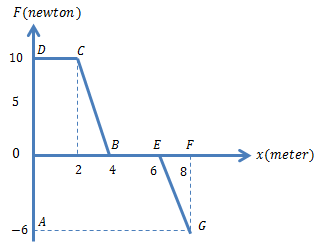
\includegraphics[width=5cm]{pic/latul-usaha4} 
\vspace{2cm}


\item Jika massa adalah 2kg, maka total usaha yang dilakukan oleh gaya gravitasi saaat bergeser 2 m adalah . . . \\
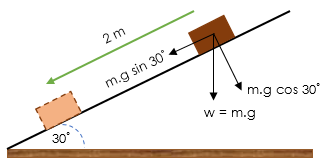
\includegraphics[width=5cm]{pic/latul-usaha3} 
\vspace{2cm}

\item Suatu balok dengan massa 2 kg berada pada ketinggian awal (perhatikan gambar). Setelah itu benda meluncur. Karena di titik A hingga B ada gaya gesek 8 N sejauh 3 m, maka balok tersebut berhenti di titik B. Berapakah besar $R$ ?
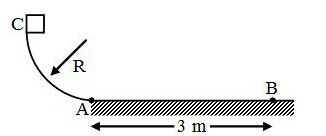
\includegraphics[width=5cm]{pic/latul-usaha2}
\vspace{3cm}

\item Peselancar meluncur dari keadaan diam seperti pada gambar. Maka kecepatan peselancar pada titik B adalah . . . \\
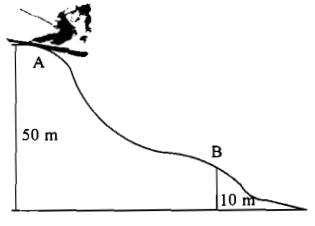
\includegraphics[width=5cm]{pic/latul-usaha1}

\end{enumerate}
\end{multicols*}\end{document}






